\textual
\chapter{Dimostrazione}

In questa sezione vengono mostrate le pagine principali dell'applicazione, sviluppate, da un punto di vista grafico, attraverso HTML e CSS, gestendo l'interazione dinamica dell'utente con Javascript e JQuery.

\section{Login Frame}

L'interfaccia di Login è minimale e presenta due input-form che vengono utilizzati per consentire all'utente di inserire l'username e la password.

\begin{figure}[!htbp]
	\centering
	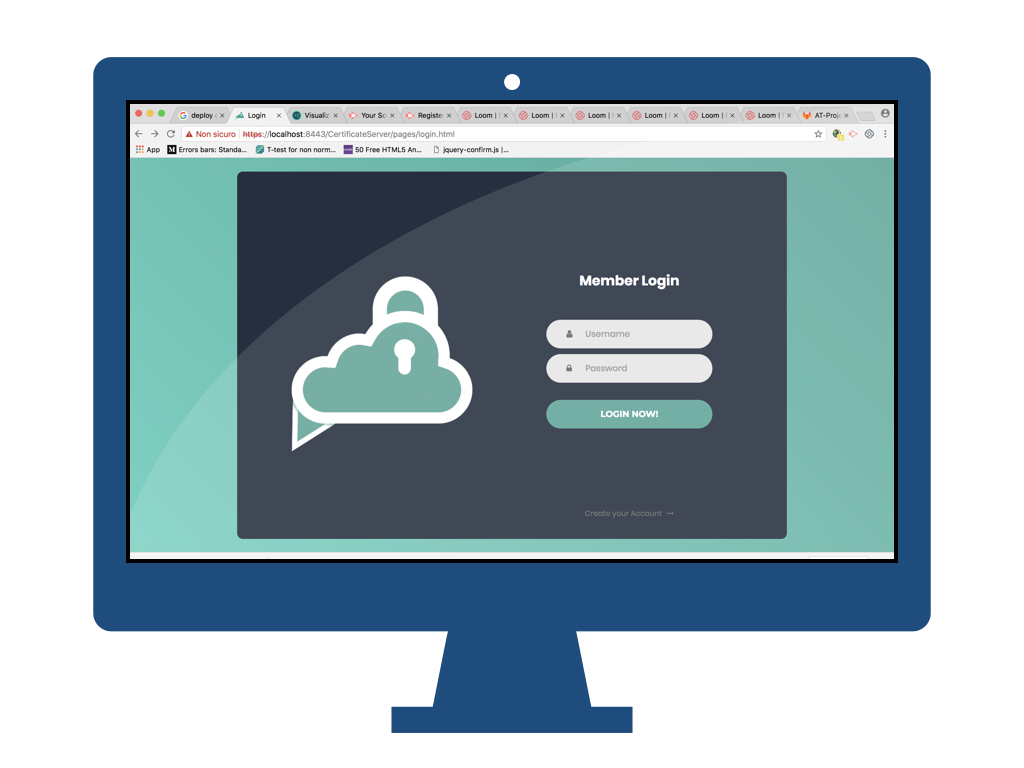
\includegraphics[scale = .3]{img/conclusioni002.jpeg}
	\caption{Scenario Login}
	\label{gfx:sdlogin}
\end{figure}

\section{Registration Frame}

L'interfaccia di Registrazione presenta input-form che vengono utilizzati per consentire all'utente di inserire l'username, la password, il nome, il cognome, l'indirizzo email e il numero di telefono. Si noti che client-side è effettuato un checking al fine di verificare che i campi non siano vuoti, che la password sia sufficientemente strong e che l'email sia ben formattata.

\begin{figure}[!htbp]
	\centering
	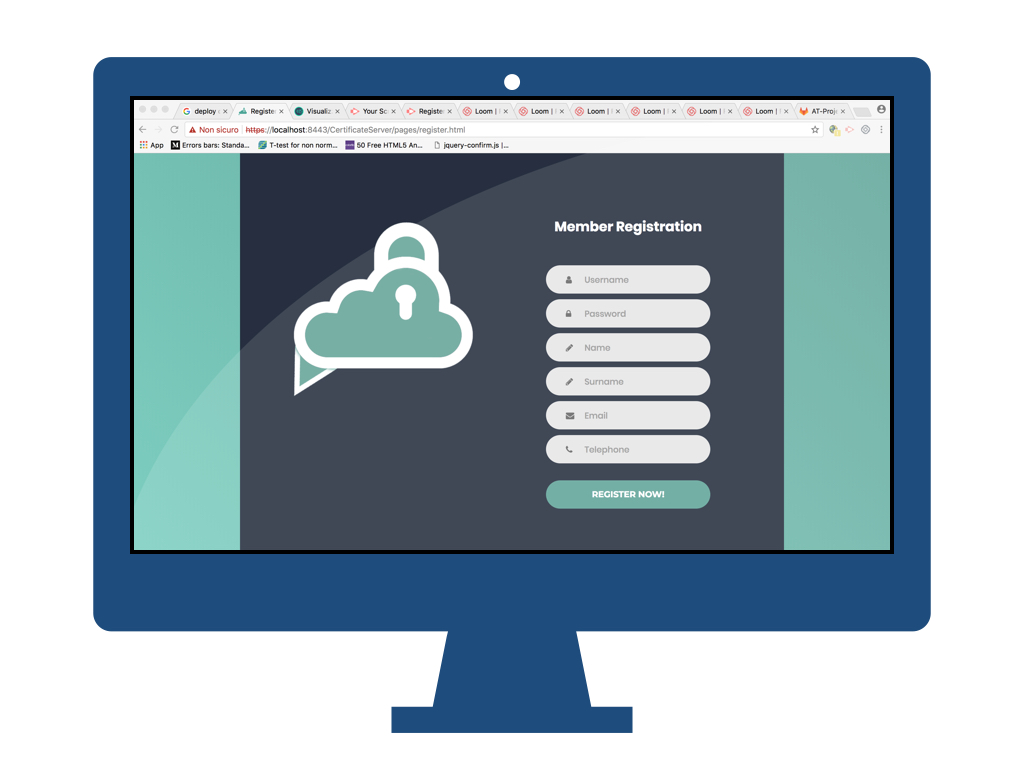
\includegraphics[scale = .3]{img/conclusioni003.jpeg}
	\caption{Scenario Registrazione}
	\label{gfx:sdregister}
\end{figure}


\section{Chat Frame}

L'interfaccia di Chat presenta una lista di contatti, opportunamente filtrata rispetto alle policy di contatto, e una finestra a destra dedicata alla chat.

\begin{figure}[!htbp]
	\centering
	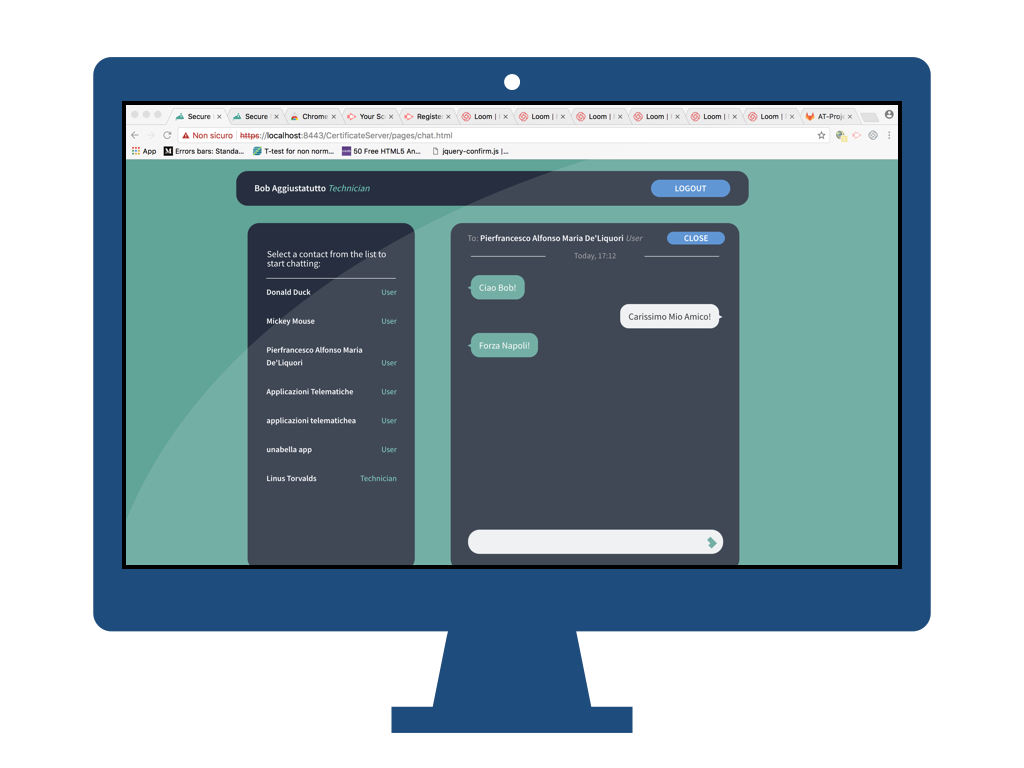
\includegraphics[scale = .3]{img/conclusioni001.jpeg}
	\caption{Scenario Chat}
	\label{gfx:sdchat}
\end{figure}
